\documentclass{ximera}

%\usepackage{todonotes}

\newcommand{\todo}{}

\usepackage{esint} % for \oiint
\ifxake%%https://math.meta.stackexchange.com/questions/9973/how-do-you-render-a-closed-surface-double-integral
\renewcommand{\oiint}{{\large\bigcirc}\kern-1.56em\iint}
\fi


\graphicspath{
  {./}
  {ximeraTutorial/}
  {basicPhilosophy/}
  {functionsOfSeveralVariables/}
  {normalVectors/}
  {lagrangeMultipliers/}
  {vectorFields/}
  {greensTheorem/}
  {shapeOfThingsToCome/}
  {dotProducts/}
  {partialDerivativesAndTheGradientVector/}
  {../productAndQuotientRules/exercises/}
  {../normalVectors/exercisesParametricPlots/}
  {../continuityOfFunctionsOfSeveralVariables/exercises/}
  {../partialDerivativesAndTheGradientVector/exercises/}
  {../directionalDerivativeAndChainRule/exercises/}
  {../commonCoordinates/exercisesCylindricalCoordinates/}
  {../commonCoordinates/exercisesSphericalCoordinates/}
  {../greensTheorem/exercisesCurlAndLineIntegrals/}
  {../greensTheorem/exercisesDivergenceAndLineIntegrals/}
  {../shapeOfThingsToCome/exercisesDivergenceTheorem/}
  {../greensTheorem/}
  {../shapeOfThingsToCome/}
  {../separableDifferentialEquations/exercises/}
  {vectorFields/}
}

\newcommand{\mooculus}{\textsf{\textbf{MOOC}\textnormal{\textsf{ULUS}}}}

\usepackage{tkz-euclide}
\usepackage{tikz}
\usepackage{tikz-cd}
\usetikzlibrary{arrows}
\tikzset{>=stealth,commutative diagrams/.cd,
  arrow style=tikz,diagrams={>=stealth}} %% cool arrow head
\tikzset{shorten <>/.style={ shorten >=#1, shorten <=#1 } } %% allows shorter vectors

\usetikzlibrary{backgrounds} %% for boxes around graphs
\usetikzlibrary{shapes,positioning}  %% Clouds and stars
\usetikzlibrary{matrix} %% for matrix
\usepgfplotslibrary{polar} %% for polar plots
\usepgfplotslibrary{fillbetween} %% to shade area between curves in TikZ
%\usetkzobj{all}
\usepackage[makeroom]{cancel} %% for strike outs
%\usepackage{mathtools} %% for pretty underbrace % Breaks Ximera
%\usepackage{multicol}
\usepackage{pgffor} %% required for integral for loops



%% http://tex.stackexchange.com/questions/66490/drawing-a-tikz-arc-specifying-the-center
%% Draws beach ball
\tikzset{pics/carc/.style args={#1:#2:#3}{code={\draw[pic actions] (#1:#3) arc(#1:#2:#3);}}}



\usepackage{array}
\setlength{\extrarowheight}{+.1cm}
\newdimen\digitwidth
\settowidth\digitwidth{9}
\def\divrule#1#2{
\noalign{\moveright#1\digitwidth
\vbox{\hrule width#2\digitwidth}}}




% \newcommand{\RR}{\mathbb R}
% \newcommand{\R}{\mathbb R}
% \newcommand{\N}{\mathbb N}
% \newcommand{\Z}{\mathbb Z}

\newcommand{\sagemath}{\textsf{SageMath}}


%\renewcommand{\d}{\,d\!}
%\renewcommand{\d}{\mathop{}\!d}
%\newcommand{\dd}[2][]{\frac{\d #1}{\d #2}}
%\newcommand{\pp}[2][]{\frac{\partial #1}{\partial #2}}
% \renewcommand{\l}{\ell}
%\newcommand{\ddx}{\frac{d}{\d x}}

% \newcommand{\zeroOverZero}{\ensuremath{\boldsymbol{\tfrac{0}{0}}}}
%\newcommand{\inftyOverInfty}{\ensuremath{\boldsymbol{\tfrac{\infty}{\infty}}}}
%\newcommand{\zeroOverInfty}{\ensuremath{\boldsymbol{\tfrac{0}{\infty}}}}
%\newcommand{\zeroTimesInfty}{\ensuremath{\small\boldsymbol{0\cdot \infty}}}
%\newcommand{\inftyMinusInfty}{\ensuremath{\small\boldsymbol{\infty - \infty}}}
%\newcommand{\oneToInfty}{\ensuremath{\boldsymbol{1^\infty}}}
%\newcommand{\zeroToZero}{\ensuremath{\boldsymbol{0^0}}}
%\newcommand{\inftyToZero}{\ensuremath{\boldsymbol{\infty^0}}}



% \newcommand{\numOverZero}{\ensuremath{\boldsymbol{\tfrac{\#}{0}}}}
% \newcommand{\dfn}{\textbf}
% \newcommand{\unit}{\,\mathrm}
% \newcommand{\unit}{\mathop{}\!\mathrm}
% \newcommand{\eval}[1]{\bigg[ #1 \bigg]}
% \newcommand{\seq}[1]{\left( #1 \right)}
% \renewcommand{\epsilon}{\varepsilon}
% \renewcommand{\phi}{\varphi}


% \renewcommand{\iff}{\Leftrightarrow}

% \DeclareMathOperator{\arccot}{arccot}
% \DeclareMathOperator{\arcsec}{arcsec}
% \DeclareMathOperator{\arccsc}{arccsc}
% \DeclareMathOperator{\si}{Si}
% \DeclareMathOperator{\scal}{scal}
% \DeclareMathOperator{\sign}{sign}


%% \newcommand{\tightoverset}[2]{% for arrow vec
%%   \mathop{#2}\limits^{\vbox to -.5ex{\kern-0.75ex\hbox{$#1$}\vss}}}
% \newcommand{\arrowvec}[1]{{\overset{\rightharpoonup}{#1}}}
% \renewcommand{\vec}[1]{\arrowvec{\mathbf{#1}}}
% \renewcommand{\vec}[1]{{\overset{\boldsymbol{\rightharpoonup}}{\mathbf{#1}}}}

% \newcommand{\point}[1]{\left(#1\right)} %this allows \vector{ to be changed to \vector{ with a quick find and replace
% \newcommand{\pt}[1]{\mathbf{#1}} %this allows \vec{ to be changed to \vec{ with a quick find and replace
% \newcommand{\Lim}[2]{\lim_{\point{#1} \to \point{#2}}} %Bart, I changed this to point since I want to use it.  It runs through both of the exercise and exerciseE files in limits section, which is why it was in each document to start with.

% \DeclareMathOperator{\proj}{\mathbf{proj}}
% \newcommand{\veci}{{\boldsymbol{\hat{\imath}}}}
% \newcommand{\vecj}{{\boldsymbol{\hat{\jmath}}}}
% \newcommand{\veck}{{\boldsymbol{\hat{k}}}}
% \newcommand{\vecl}{\vec{\boldsymbol{\l}}}
% \newcommand{\uvec}[1]{\mathbf{\hat{#1}}}
% \newcommand{\utan}{\mathbf{\hat{t}}}
% \newcommand{\unormal}{\mathbf{\hat{n}}}
% \newcommand{\ubinormal}{\mathbf{\hat{b}}}

% \newcommand{\dotp}{\bullet}
% \newcommand{\cross}{\boldsymbol\times}
% \newcommand{\grad}{\boldsymbol\nabla}
% \newcommand{\divergence}{\grad\dotp}
% \newcommand{\curl}{\grad\cross}
%\DeclareMathOperator{\divergence}{divergence}
%\DeclareMathOperator{\curl}[1]{\grad\cross #1}
% \newcommand{\lto}{\mathop{\longrightarrow\,}\limits}

% \renewcommand{\bar}{\overline}

\colorlet{textColor}{black}
\colorlet{background}{white}
\colorlet{penColor}{blue!50!black} % Color of a curve in a plot
\colorlet{penColor2}{red!50!black}% Color of a curve in a plot
\colorlet{penColor3}{red!50!blue} % Color of a curve in a plot
\colorlet{penColor4}{green!50!black} % Color of a curve in a plot
\colorlet{penColor5}{orange!80!black} % Color of a curve in a plot
\colorlet{penColor6}{yellow!70!black} % Color of a curve in a plot
\colorlet{fill1}{penColor!20} % Color of fill in a plot
\colorlet{fill2}{penColor2!20} % Color of fill in a plot
\colorlet{fillp}{fill1} % Color of positive area
\colorlet{filln}{penColor2!20} % Color of negative area
\colorlet{fill3}{penColor3!20} % Fill
\colorlet{fill4}{penColor4!20} % Fill
\colorlet{fill5}{penColor5!20} % Fill
\colorlet{gridColor}{gray!50} % Color of grid in a plot

\newcommand{\surfaceColor}{violet}
\newcommand{\surfaceColorTwo}{redyellow}
\newcommand{\sliceColor}{greenyellow}




\pgfmathdeclarefunction{gauss}{2}{% gives gaussian
  \pgfmathparse{1/(#2*sqrt(2*pi))*exp(-((x-#1)^2)/(2*#2^2))}%
}


%%%%%%%%%%%%%
%% Vectors
%%%%%%%%%%%%%

%% Simple horiz vectors
\renewcommand{\vector}[1]{\left\langle #1\right\rangle}


%% %% Complex Horiz Vectors with angle brackets
%% \makeatletter
%% \renewcommand{\vector}[2][ , ]{\left\langle%
%%   \def\nextitem{\def\nextitem{#1}}%
%%   \@for \el:=#2\do{\nextitem\el}\right\rangle%
%% }
%% \makeatother

%% %% Vertical Vectors
%% \def\vector#1{\begin{bmatrix}\vecListA#1,,\end{bmatrix}}
%% \def\vecListA#1,{\if,#1,\else #1\cr \expandafter \vecListA \fi}

%%%%%%%%%%%%%
%% End of vectors
%%%%%%%%%%%%%

%\newcommand{\fullwidth}{}
%\newcommand{\normalwidth}{}



%% makes a snazzy t-chart for evaluating functions
%\newenvironment{tchart}{\rowcolors{2}{}{background!90!textColor}\array}{\endarray}

%%This is to help with formatting on future title pages.
\newenvironment{sectionOutcomes}{}{}



%% Flowchart stuff
%\tikzstyle{startstop} = [rectangle, rounded corners, minimum width=3cm, minimum height=1cm,text centered, draw=black]
%\tikzstyle{question} = [rectangle, minimum width=3cm, minimum height=1cm, text centered, draw=black]
%\tikzstyle{decision} = [trapezium, trapezium left angle=70, trapezium right angle=110, minimum width=3cm, minimum height=1cm, text centered, draw=black]
%\tikzstyle{question} = [rectangle, rounded corners, minimum width=3cm, minimum height=1cm,text centered, draw=black]
%\tikzstyle{process} = [rectangle, minimum width=3cm, minimum height=1cm, text centered, draw=black]
%\tikzstyle{decision} = [trapezium, trapezium left angle=70, trapezium right angle=110, minimum width=3cm, minimum height=1cm, text centered, draw=black]


\title{Graph Movement}

\begin{document}

\begin{abstract}
horizontal
\end{abstract}
\maketitle




\textbf{\textcolor{purple}{$\star$ Composition with a linear function as the inside function results in horizontal graphical transformations.}}






Let $W(t) = 3 |t-1| - 3$ with domain $[-1, 5)$.





\begin{image}
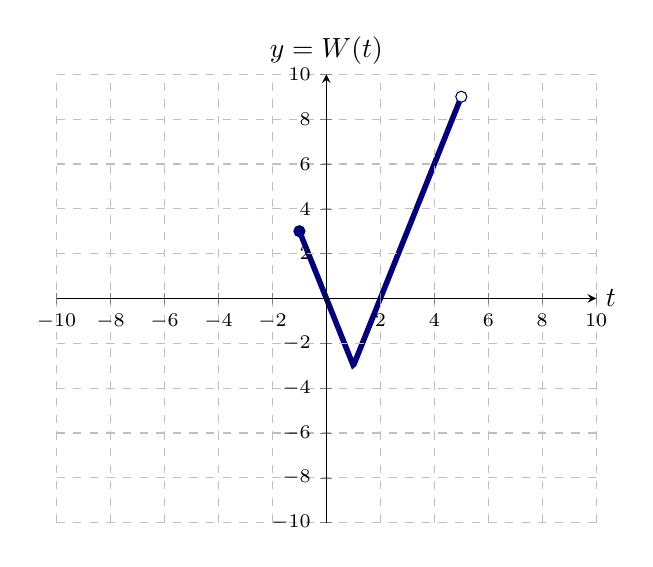
\begin{tikzpicture}
  \begin{axis}[
            domain=-10:10, ymax=10, xmax=10, ymin=-10, xmin=-10,
            axis lines =center, xlabel=$t$, ylabel={$y=W(t)$}, grid = major, grid style={dashed},
            ytick={-10,-8,-6,-4,-2,2,4,6,8,10},
            xtick={-10,-8,-6,-4,-2,2,4,6,8,10},
            yticklabels={$-10$,$-8$,$-6$,$-4$,$-2$,$2$,$4$,$6$,$8$,$10$}, 
            xticklabels={$-10$,$-8$,$-6$,$-4$,$-2$,$2$,$4$,$6$,$8$,$10$},
            ticklabel style={font=\scriptsize},
            every axis y label/.style={at=(current axis.above origin),anchor=south},
            every axis x label/.style={at=(current axis.right of origin),anchor=west},
            axis on top
          ]
          
            
      		\addplot [line width=2, penColor, smooth,samples=200,domain=(-1:5)] {3*abs(x-1) - 3};

      		\addplot[color=penColor,fill=penColor,only marks,mark=*] coordinates{(-1,3)};
      		\addplot[color=penColor,fill=white,only marks,mark=*] coordinates{(5,9)};






  \end{axis}
\end{tikzpicture}
\end{image}



\textbf{Briefly:} $t$ moves along the real line left to right from $-1$ to $5$. We first encounter an included endpoint and then a short line segment, then a corner at $1$, then a longer line segment with an excluded endpoint. \\







$\blacktriangleright$ And, now compose it with $L(x) = -\frac{1}{2}x$ \\



$(W \circ L)(z) = W(L(z))$



\begin{explanation}

We have three functions: $W$, $L$, and $W \circ L$.  We would like to keep these separate in our thoughts.  Therefore, we will have three separate variables representing their dmomains.


\begin{itemize}
\item $W(t)$
\item $L(x)$
\item $(W \circ L)(z) = W(L(z))$
\end{itemize}

\end{explanation}






The implied, natural domain for $L$ is \textbf{$\mathbb{R}$}.  The natural range for $L$ is \textbf{$\mathbb{R}$}. This does not match the domain of $W$.  


\begin{question}


The domain of $W$ is only $\left[ \answer{-1}, \answer{5} \right)$. 

\end{question}

Therefore, we must align those.

But, before doing that, let's just think about traversing the real number line. \\

We can imagine $x$ moving along the real line left to right from $-\infty$ to $\infty$. These numbers are input into $L$ and the output runs right to left from $\infty$ to $-\infty$.  The direction is reversed because of the $-\frac{1}{2}$ coefficient in $L$.  It is changing the sign of the numbers.


Therefore, in the composition, the domain of $W$ is running backwards.  From right to left, the composition will first encounter the longer line segment with the excluded endpoint, then a corner, then the shorter line segment with the included endpoint.

The graph is reflected horizontally. \\


That was due to the negative sign of the coefficient.  Now to figure out the effect of $\frac{1}{2}$, which is less than $1$.


The domain of $W$ is $[-1, 5)$.  So, when do the values of $L(x)$ equal $-1$ and $5$ in the range?  



\begin{question}

Since all of the domain numbers of $L$ are multiplied by $-\frac{1}{2}$, these function values, $-1$ and $5$, of $L$ occur at $\answer{2}$ and $\answer{-10}$ in the domain of $L$. \\

\end{question}


The domain of $W \circ L$ is $(-10, 2]$. \\



$z$ will move across the interval $(-10, 2]$, from left to right.  \\

These domain values will be multiplied by $-\frac{1}{2}$ and the function values of $L$ will move across the interval $[-1, 5)$ from right to left.  These values are going into $W$ backwards from their normal order.

The graph of $W \circ L$ will first encounter the longer line segment with the excluded endpoint, then it will cross the corner.  

\begin{question}

The corner occurs at $ t = \answer{1}$ in the domain of $W$, which is the range of $L$. In $L$, $1$ occurs at $\answer{-2}$, in the domain of $L$.  \\

\end{question}

Then the graph of $W \circ L$ encounters the shorter line segment with the included endpoint. \\





Let $(W \circ L)(z) = 3 |-\frac{1}{2}z-1| - 3$ with domain $(-10, 2]$.


\begin{image}
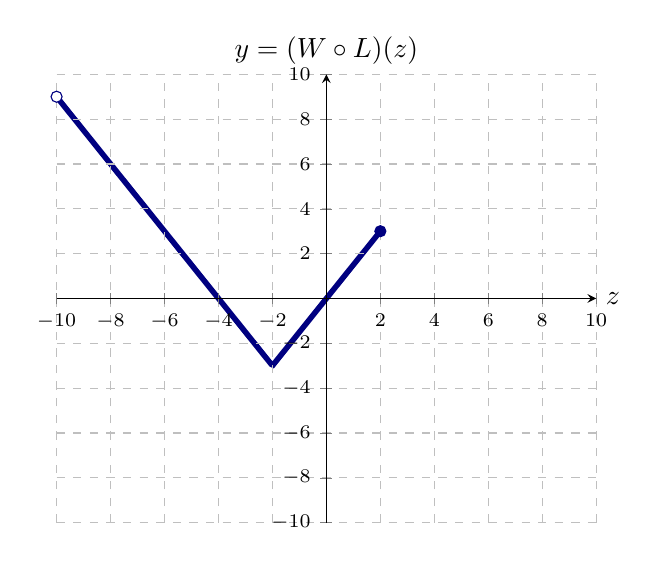
\begin{tikzpicture}
  \begin{axis}[
            domain=-10:10, ymax=10, xmax=10, ymin=-10, xmin=-10,
            axis lines =center, xlabel=$z$, ylabel={$y=(W \circ L)(z)$}, grid = major, grid style={dashed},
            ytick={-10,-8,-6,-4,-2,2,4,6,8,10},
            xtick={-10,-8,-6,-4,-2,2,4,6,8,10},
            yticklabels={$-10$,$-8$,$-6$,$-4$,$-2$,$2$,$4$,$6$,$8$,$10$}, 
            xticklabels={$-10$,$-8$,$-6$,$-4$,$-2$,$2$,$4$,$6$,$8$,$10$},
            ticklabel style={font=\scriptsize},
            every axis y label/.style={at=(current axis.above origin),anchor=south},
            every axis x label/.style={at=(current axis.right of origin),anchor=west},
            axis on top
          ]
          
            
      		\addplot [line width=2, penColor, smooth,samples=200,domain=(-10:2)] {3*abs(-0.5*x-1) - 3};

      		\addplot[color=penColor,fill=penColor,only marks,mark=*] coordinates{(2,3)};
      		\addplot[color=penColor,fill=white,only marks,mark=*] coordinates{(-10,9)};






  \end{axis}
\end{tikzpicture}
\end{image}


The graph has transformed horizontally. \\


\begin{itemize}
\item The negative coefficient in $L$ has reflected the graph horizontally.
\item The $\frac{1}{2}$ coefficient means the domain needs to expand by a factor of $2$, so that the values of $L$ match the normal inputs to $W$.
\end{itemize}


\begin{question}

The corner of the graph of an absolute value function occurs when the inside of the absolute value signs equal $\answer{0}$.


For $W$, this means $-\frac{1}{2}z-1 = 0$, which occurs when $z = \answer{-2}$. 

The corner on the graph is $\left( \answer{-2}, \answer{-3} \right)$

\end{question}

















\begin{example}


Let $F(x) = 5 \sqrt{x + 3} - 6$ with its natural or implied domain.





\begin{image}
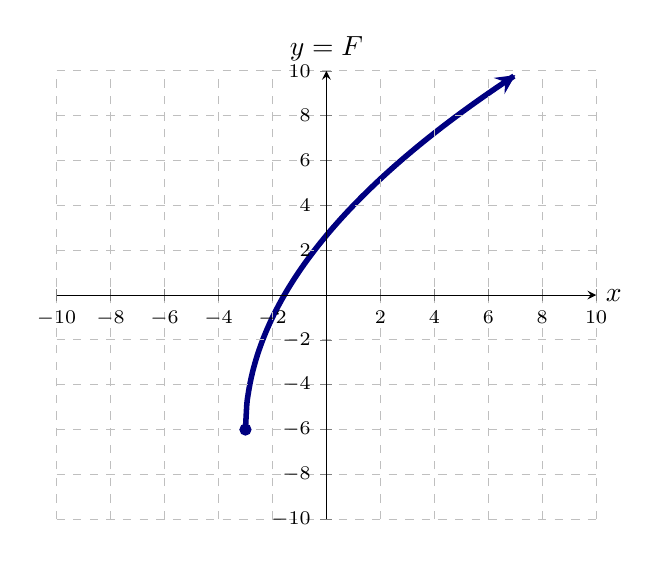
\begin{tikzpicture}
  \begin{axis}[
            domain=-10:10, ymax=10, xmax=10, ymin=-10, xmin=-10,
            axis lines =center, xlabel=$x$, ylabel={$y=F$}, grid = major, grid style={dashed},
            ytick={-10,-8,-6,-4,-2,2,4,6,8,10},
            xtick={-10,-8,-6,-4,-2,2,4,6,8,10},
            yticklabels={$-10$,$-8$,$-6$,$-4$,$-2$,$2$,$4$,$6$,$8$,$10$}, 
            xticklabels={$-10$,$-8$,$-6$,$-4$,$-2$,$2$,$4$,$6$,$8$,$10$},
            ticklabel style={font=\scriptsize},
            every axis y label/.style={at=(current axis.above origin),anchor=south},
            every axis x label/.style={at=(current axis.right of origin),anchor=west},
            axis on top
          ]
          
            
          \addplot [line width=2, penColor, smooth,samples=200,domain=(-3:7), ->] {5 * (x + 3)^0.5 - 6};

          \addplot[color=penColor,fill=penColor,only marks,mark=*] coordinates{(-3,-6)};
          %\addplot[color=penColor,fill=white,only marks,mark=*] coordinates{(-10,9)};






  \end{axis}
\end{tikzpicture}
\end{image}



\textbf{Feature Inventory:} 


\begin{itemize}
\item Domain is $\left[ \answer{-3}, \infty \right)$.
\item Starting point is $\left( -3, \answer{-6} \right)$.
\item Graph opens to the right.
\item $F$ is an increasing function.
\end{itemize}



Since, $F$ is an increasing function, there should be one zero.

\begin{align*}
5 \sqrt{x + 3} - 6 &= \answer{0} \\
5 \sqrt{x + 3}     &= 6 \\
\sqrt{x + 3}       &= \frac{6}{5} \\
\answer{x + 3}              &= \frac{36}{25}  \\
x                  &= \frac{36}{25} - 3 \\
x                  &= \frac{-39}{25} \approx -1.56
\end{align*}




$\blacktriangleright$ Now a Composition


Let $L(t) = 2t - 3$ with its natural or implied domain. \\


Define $C(z) = F(L(z))$ with its natural or implied domain. \\

\[
C(z) = F(L(z)) = 5 \sqrt{(2z - 3) + 3} - 6 
\]



$L$ will be taking real numbers and doing this to them: $2t - 3$.  \textbf{AFTER} it does that, the values will go into $F$ and at this time they need to match up to our inventory list.

Therefore, to locate all of the corresponding places in the domain of $F \circ L$ we must undo $2t - 3$.

\begin{itemize}
\item add $3$
\item multiply by $\frac{1}{2}$
\end{itemize}

The starting point is now $((-3 + 3)\cdot \frac{1}{2}, -6) = \left( \answer{0}, -6 \right)$.

The zero is now at $\left( \frac{-39}{25} + 3 \right) \cdot \frac{1}{2} = \answer{\frac{18}{25}} \approx 0.72$








\begin{image}
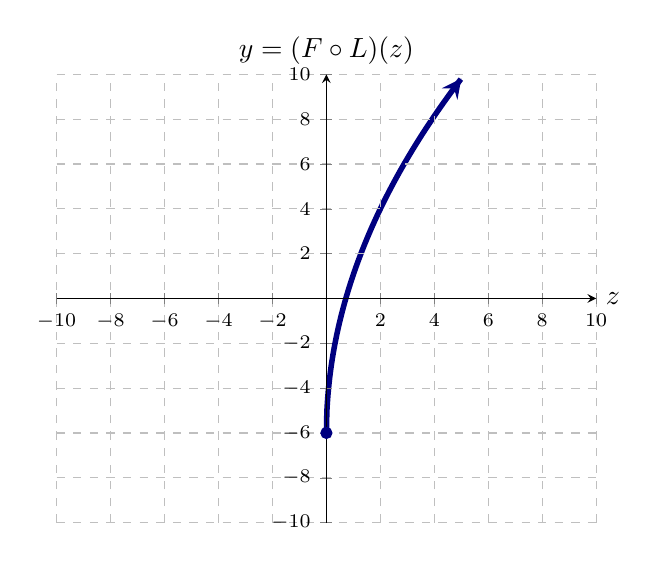
\begin{tikzpicture}
  \begin{axis}[
            domain=-10:10, ymax=10, xmax=10, ymin=-10, xmin=-10,
            axis lines =center, xlabel=$z$, ylabel={$y=(F \circ L)(z)$}, grid = major, grid style={dashed},
            ytick={-10,-8,-6,-4,-2,2,4,6,8,10},
            xtick={-10,-8,-6,-4,-2,2,4,6,8,10},
            yticklabels={$-10$,$-8$,$-6$,$-4$,$-2$,$2$,$4$,$6$,$8$,$10$}, 
            xticklabels={$-10$,$-8$,$-6$,$-4$,$-2$,$2$,$4$,$6$,$8$,$10$},
            ticklabel style={font=\scriptsize},
            every axis y label/.style={at=(current axis.above origin),anchor=south},
            every axis x label/.style={at=(current axis.right of origin),anchor=west},
            axis on top
          ]
          
            
          \addplot [line width=2, penColor, smooth,samples=300,domain=(0:5), ->] {5 * ((2*x-3) + 3)^0.5 - 6};

          \addplot[color=penColor,fill=penColor,only marks,mark=*] coordinates{(0,-6)};
          %\addplot[color=penColor,fill=white,only marks,mark=*] coordinates{(-10,9)};






  \end{axis}
\end{tikzpicture}
\end{image}





We also know that the graphs of square root functions begin when the inside equals $0$. 

\[
C(z) = F(L(z)) = 5 \sqrt{(2z - 3) + 3} - 6 = 5 \sqrt{2z} - 6
\]


Beginning at $2z = 0$ or $z = 0$. \\

$C$ has a zero, for which we can just solve.




\begin{align*}
5 \sqrt{2z} - 6 &= 0 \\
5 \sqrt{2z}     &= 6 \\
\sqrt{2z}       &= \frac{6}{5} \\
2z            &= \frac{36}{25}  \\
z                  &= \frac{36}{50} \\
z                 &= \frac{18}{25} \approx 0.72
\end{align*}




\end{example}




















\begin{center}
\textbf{\textcolor{green!50!black}{ooooo-=-=-=-ooOoo-=-=-=-ooooo}} \\

more examples can be found by following this link\\ \link[More Examples of Transforming the Inside]{https://ximera.osu.edu/csccmathematics/precalculus1/precalculus1/transformationsInside/examples/exampleList}

\end{center}




\end{document}
